%!TEX TS-program = xelatex
\documentclass[]{friggeri-cv}
\usepackage{afterpage}
\usepackage{hyperref}
\usepackage{color}
\usepackage{xcolor}

\hypersetup{
    pdftitle={},
    pdfauthor={},
    pdfsubject={},
    pdfkeywords={},
    colorlinks=false,       % no lik border color
   allbordercolors=white    % white border color for all
}
\addbibresource{bibliography.bib}
\RequirePackage{xcolor}
\definecolor{pblue}{HTML}{0395DE}

\begin{document}
\header{I}{DEAR}
      {硕士研究生}
      
% Fake text to add separator      
\fcolorbox{white}{gray}{\parbox{\dimexpr\textwidth-2\fboxsep-2\fboxrule}{%
.....
}}

% In the aside, each new line forces a line break
\begin{aside}
  \section{现居地址}
    苯丙酮尿大学男生院
    北京市海淀区
    颐和园路5号%,100871
    ~
  \section{手机号码}
    110120119
    ~
  \section{电子邮箱}
    \href{mailto:wangdongwei@pku.edu.cn}{\textbf{wangdongwei@}\\pku.edu.cn}
    \href{mailto:wangdongwei1203@gmail.com}{\textbf{wangdongwei1203@}\\gmail.com}
    ~
  \section{Git}
    %需要考虑创建个网址
    \href{https://github.com/idear1}{github.com/idear1}
    ~
  \section{编程语言}
    ~
    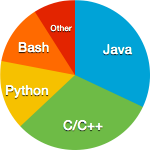
\includegraphics[scale=0.7]{img/programming.png}
    ~
  \section{操作系统偏好}
    \textbf{MacOS}
\includegraphics[scale=0.40]{img/5stars.png}
    \textbf{GNU/Linux}
\includegraphics[scale=0.40]{img/4stars.png}
    \textbf{Windows}
\includegraphics[scale=0.40]{img/1stars.png}
    ~
  \section{语言能力}
    \textbf{英语}
\includegraphics[scale=0.40]{img/4stars.png}
    ~
\end{aside}

\section{教育经历}
\begin{entrylist}
  \entry
    {14/09 至今}
    {拖拉机专业,硕士研究生}
    {苯丙酮尿大学}
    {研究方向:勾搭妹子\\
    主要课程:软件卖萌技术, 软件逗逼模式\\
    }
  \entry
    {10/09 - 14/06}
    {蜘蛛网专业,工科学士学位}
    {北京没电大学}
    {
    主要课程: 低级卖萌技术,低级逗逼模式
    }
\end{entrylist}

\section{工作经历}
\begin{entrylist}
  \entry
    {13/09 至今 }
    {程序猿}
    {某中心}
    {吃\\
    喝\\
    玩\\
    乐\\}

  \entry
    {11/10 - 12/07}
    {码农}
    {某实验室}
    {打杂\\
    搬砖}
\end{entrylist}


\section{获奖经历}
\begin{entrylist}
  \entry
    {14/10}
    {最佳卖萌奖}
    {校级}
    {\emph{此处应有说明}\\}

  \entry
    {14/06}
    {最逗逼奖}
    {国家级}
    {\emph{啊啊啊,黑猫警长
    }}
\end{entrylist}


\newpage

\begin{aside}
~
~
~
  \section{MBTI职业性格}
  ~
    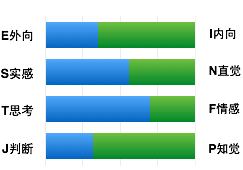
\includegraphics[scale=0.5]{img/personal.png}
    ~
\end{aside}

%\begin{entrylist}
%entrylist默认是不分页的。我没有找到好的解决方案。我的做法是手动增加一个entrylist,反正简历不会太长。
%\end{entrylist}
~
\section{论文发表}
小明,小白,小粉,我.
\textbf{车辆工程与软件工程的交叉研究}.\emph{某学报,1991,43(4),234-322}
\\
\section{其他信息}
\begin{enumerate}
\item 会做饭,会暖床,单身,性别男,爱好女。女神不从。
\item 熟悉\LaTeX 排版技术。
\end{enumerate}

\section{大众评价}
\begin{enumerate}
\item IDEAR的忠实粉丝夏同学:手中无码,心中有码。华北地区第一码神,行云流水,腾云驾雾。他的代码作品,有如窈窕淑女,出水芙蓉,绕梁三日,令人乐不思蜀,久久无法自拔。
\item 苹果总裁库克:我多么希望Apple的工程师能有IDEAR哪怕十分之一的天赋。
\item 伊力诺斯大学LLVM/Clang项目总监:每当IDEAR的代码无法通过Clang的编译时,我就知道我们该修改这该死的编译器了。
\item 非诚勿扰节目主持人乐嘉:幸好我不是女嘉宾,否则除了电击失忆治疗以外,只有爱上IDEAR,别无选择。
\end{enumerate}


%%% This piece of code has been commented by Karol Kozio艂 due to biblatex errors. 
% 
%\printbibsection{article}{article in peer-reviewed journal}
%\begin{refsection}
%  \nocite{*}
%  \printbibliography[sorting=chronological, type=inproceedings, title={international peer-reviewed conferences/proceedings}, notkeyword={france}, heading=subbibliography]
%\end{refsection}
%\begin{refsection}
%  \nocite{*}
%  \printbibliography[sorting=chronological, type=inproceedings, title={local peer-reviewed conferences/proceedings}, keyword={france}, heading=subbibliography]
%\end{refsection}
%\printbibsection{misc}{other publications}
%\printbibsection{report}{research reports}

\end{document}
